\documentclass{article}
\special{papersize=8.5in,11in}
\usepackage[top=1in, bottom=1in, left=1in, right=1in]{geometry}
% \usepackage{fullpage, fancyhdr}
\usepackage{fullpage}
\usepackage{float}
\usepackage{mathtools}
\usepackage{caption}
\usepackage{sidecap} % enable side captions
\usepackage{subcaption}
\usepackage{portland}
\usepackage{graphicx}
\setlength{\topmargin}{0.0in}
\setlength{\headheight}{0.5in}
\setlength{\headsep}{0in}
\setlength{\footskip}{9pt}

% General tikz + pgf-umlsd
\usepackage{wrapfig}
\usepackage{listings}
\usepackage{tikz}
\usepackage{pgf-umlsd}
\usepgflibrary{arrows}
\usetikzlibrary{shapes,arrows,shadows}
\usetikzlibrary{shapes.geometric}

\DeclareMathAlphabet{\mathpzc}{OT1}{pzc}{m}{it}
\newcommand{\z}{\mathpzc{z}}

% Use so that included code is pretty
\usepackage{listings}
\usepackage{color}

\definecolor{dkgreen}{rgb}{0,0.6,0}
\definecolor{gray}{rgb}{0.5,0.5,0.5}
\definecolor{mauve}{rgb}{0.58,0,0.82}

\lstset{ %
  backgroundcolor=\color{white},  % choose the background color; you must add \usepackage{color} or \usepackage{xcolor}
  basicstyle=\footnotesize,       % the size of the fonts that are used for the code
  breakatwhitespace=false,        % sets if automatic breaks should only happen at whitespace
  breaklines=true,                % sets automatic line breaking
  captionpos=t,                   % sets the caption-position to bottom
  commentstyle=\color{dkgreen},   % comment style
%   deletekeywords={...},           % if you want to delete keywords from the given language
%   escapeinside={\%*}{*)},         % if you want to add LaTeX within your code
%   extendedchar=false,             % lets you use non-ASCII characters; for 8-bits encodings only, does not work with UTF-8
  frame=single,                   % adds a frame around the code
  keywordstyle=\color{blue},      % keyword style
  language={[x86masm]Assembler},                % the language of the code
  morekeywords={LDR,AREA,ENTRY,CODE,DATA,DCD,SPACE,BLT,B,BL.W,ADDS,VMOV,IN,ZAP,MAC,APAC,ADD,SACH,MACD,OUT,},           % if you want to add more keywords to the set
  numbers=left,                   % where to put the line-numbers; possible values are (none, left, right)
  numbersep=5pt,                  % how far the line-numbers are from the code
  numberstyle=\tiny\color{gray},  % the style that is used for the line-numbers
  rulecolor=\color{black},        % if not set, the frame-color may be changed on line-breaks within not-black text (e.g. comments (green here))
  showspaces=false,               % show spaces everywhere adding particular underscores; it overrides 'showstringspaces'
  showstringspaces=false,         % underline spaces within strings only
  showtabs=false,                 % show tabs within strings adding particular underscores
  stepnumber=1,                   % the step between two line-numbers. If it's 1, each line will be numbered
  stringstyle=\color{mauve},      % string literal style
  tabsize=8,                      % sets default tabsize to 2 spaces
  title=\lstname                  % show the filename of files included with \lstinputlisting; also try caption instead of title
}



% \pagestyle{fancyplain}
\pagestyle{myheadings}
\voffset=-0.50in
\topmargin=0.00in 
\headsep=0.25in 
\evensidemargin=0in 
\oddsidemargin=0in 
\textwidth=6.6in 
\textheight=10.0in 

\renewcommand{\topfraction}{0.9}	% max fraction of floats at top
\renewcommand{\bottomfraction}{0.8}	% max fraction of floats at bottom
%   Parameters for TEXT pages (not float pages):
\setcounter{topnumber}{2}
\setcounter{bottomnumber}{2}
\setcounter{totalnumber}{4}     % 2 may work better
\setcounter{dbltopnumber}{2}    % for 2-column pages
\renewcommand{\dbltopfraction}{0.9}	% fit big float above 2-col. text
\renewcommand{\textfraction}{0.07}	% allow minimal text w. figs
%   Parameters for FLOAT pages (not text pages):
\renewcommand{\floatpagefraction}{0.7}	% require fuller float pages
% N.B.: floatpagefraction MUST be less than topfraction !!
\renewcommand{\dblfloatpagefraction}{0.7}	% require fuller float pages
% remember to use [htp] or [htpb] for placement

\title{Assignment \# 7: Problem Set 4, Problem 2}
\date{2/15/2013}
\author{Brian Arnberg}

\markright{Brian Arnberg\hfill ELEC 6260 - Embedded Computing Systems\hfill}     
\setlength{\parindent}{0pt}


\renewcommand{\figurename}{\bf Q3 -}


\begin{document}\label{start}

\tikzstyle{endpoint} = [circle, draw, text width=1.8em, text centered, rounded corners, minimum height=1.8em]
\tikzstyle{block} = [rectangle, draw, text width=12.3em, text centered, rounded corners, minimum height=2em]
\tikzstyle{decision} = [diamond, draw, text width=4.5em, text badly centered, node distance=1.9cm, inner sep=0pt]
\tikzstyle{line} = [draw, -latex']

% \begin{titlepage}
	\maketitle
	\thispagestyle{empty}
% \end{titlepage}

% \section*{Assignment \# 7: Problem Set 4, Problem 2 - Due 2/15/2013}
At the end of Chapter 3, answer/work the following, which deal with input/output operations:\\
Q3-6, Q3-8, Q3-9, Q3-12, Q3-12, Q3-13, Q3-15, Q3-16, Q3-19.

% -----------------------------------------------%
% ---------   Q3-6   ----------------------------%      
\setcounter{figure}{5}
\begin{figure}[h]
	\centering
\caption{Draw a UML sequence diagram for a busy-wait read of a device. The diagram should include the program running on the CPU and the device.}
\begin{sequencediagram}
	\newthread{c}{:CPU}
	\newinst[1]{p}{:PollDevice}
	\newthread{d}{:Device}
	\begin{sdblock}{Main Loop}{}
		\begin{call}{c}{poll()}{p}{ready}
			\begin{sdblock}{Wait for Device}{}
				\mess{d}{Ready()}{p}
			\end{sdblock}
		\end{call}
	\begin{call}{c}{read()}{d}{value}
	\end{call}
	\end{sdblock}
\end{sequencediagram}
\end{figure}

% -----------------------------------------------%
% ---------   Q3-8   ----------------------------%      
\setcounter{figure}{7}
\begin{figure}[th]
\centering
\caption{Draw a UML sequence diagram for copying characters from an input to an output device using busy-wait I/O. The diagram should include the two devices and the two busy-wait I/O handlers.}
\begin{sequencediagram}
	\newthread{f}{:Foreground}
	\newinst[1]{ih}{:InputHandler}
	\newthread{id}{:InputDevice}
	\newinst[1]{oh}{:OutputHandler}
	\newthread{od}{:OutputDevice}
	\begin{sdblock}{Main Loop}{}
		\begin{call}{f}{getChar()}{ih}{char}
			\begin{sdblock}{Wait for Device}{} 
				\mess{id}{InputReady()}{ih}
			\end{sdblock}
			\begin{call}{ih}{ReadInput()}{id}{char}
			\end{call}
		\end{call}
		\begin{call}{f}{writeChar()}{oh}{}
			\begin{sdblock}{Wait for Device}{}
				\mess{od}{OutputReady()}{oh}
			\end{sdblock}
			\begin{call}{oh}{writeOutput()}{od}{}
			\end{call}
		\end{call}
	\end{sdblock}
\end{sequencediagram}
\end{figure}

% -----------------------------------------------%
% ---------   Q3-9   ----------------------------%      
\setcounter{figure}{8}
\begin{figure}[h]
	\centering
	\caption{When would you prefer to use busy-wait I/O over interrupt driven I/O?\\
	\emph{Answer:} One would prefer busy-wait I/O over interrupt driven I/O in situations wherein the main program cannot function until a device is ready to service. For instance, a calculator should wait for user input before it does anything, and once it has calculated (and displayed) the output, it should wait for more user input.  }
\end{figure}

% -----------------------------------------------%
% ---------   Q3-12  ----------------------------%      
\setcounter{figure}{11}
\begin{figure}[h]
	\centering
	\caption{Draw a UML sequence diagram for an interrupt-driven write of a device. The diagram should include the background program, the handler, and the device.}
\begin{sequencediagram}
	\newthread{c}{:CPU}
	\newinst[2]{b}{:Background}
	\newinst[1]{i}{:Interrupt Handler}
	\newthread{d}{:Device}
	\begin{call}{c}{Background}{b}{Save Contex}
		\mess{d}{Interrupt}{c}
		\begin{callself}{c}{Determine Source}{}
		\end{callself}
	\end{call}
	\begin{call}{c}{Process Interrupt}{i}{Restore Context}
		\begin{call}{i}{Write}{d}{}
		\end{call}
	\end{call}
	\begin{messcall}{c}{Return to Background}{b}
	\end{messcall}
\end{sequencediagram}

\end{figure}

% -----------------------------------------------%
% ---------   Q3-13  ----------------------------%      
\setcounter{figure}{12}
\begin{figure}[h]
	\centering
	\caption{Draw a UML sequency diagram for a vectored interrupt-driven read of a device. The diagram should include the background program, the interrupt vector table, the handler, and the device.}
\begin{sequencediagram}
	\newthread{c}{:CPU}
	\newinst[2]{b}{:Background}
	\newinst{v}{:Interrupt Vectors}
	\newinst{i}{:Interrupt Handler}
	\newthread{d}{:Device}
	\begin{call}{c}{Background}{b}{Save Current Context}
		\mess{d}{Interrupt}{c}
		\begin{callself}{c}{Determine Source}{}
		\end{callself}
	\end{call}
	\begin{call}{c}{Get Interrupt Vector}{v}{Vector}
	\end{call}
	\begin{call}{c}{Process Interrupt}{i}{Restore Context}
		\begin{call}{i}{Read}{d}{}
		\end{call}
	\end{call}
	\begin{messcall}{c}{Return to Background}{b}
	\end{messcall}

\end{sequencediagram}
\end{figure}


% -----------------------------------------------%
% ---------   Q3-15  ----------------------------%      
\setcounter{figure}{14}
\begin{figure}[h]
	\centering
	\caption{Draw a UML sequence diagram of a higher-priority interrupt that happens during a lower-priority interrupt handler. The diagram should include the device, the two handlers, and the background program.} 
\begin{sequencediagram}	
	\newthread{c}{:CPU}
	\newinst[2]{b}{:Background}
	\newinst{i1}{:Handler 1 (Higher Priority)}
	\newinst{i2}{:Handler 2}
	\newthread{d}{:Device}

	\begin{messcall}{c}{Background}{b}{}
		\mess{d}{Interrupt 2}{c}
		\begin{callself}{c}{Determine Source}{2}
		\end{callself}
		\begin{callself}{c}{Save Context}{}
		\end{callself}
	\end{messcall}

	\begin{messcall}{c}{Handle Interrupt 2}{i2}{}
		\begin{callself}{i2}{Start}{}
		\end{callself}
		\mess{d}{Interrupt 1}{c}
		\begin{callself}{c}{Determine Source}{1}
		\end{callself}
		\begin{callself}{c}{Save Context}{}
		\end{callself}
	\end{messcall}

	\begin{call}{c}{Handle Interrupt 1}{i1}{Restore Context}
		\begin{callself}{i1}{Execute Everything}{}
		\end{callself}
	\end{call}

	\begin{call}{c}{Return to Interrupt 2}{i2}{Restore Context}
		\begin{callself}{i2}{Finish}{}
		\end{callself}
	\end{call}

	\begin{messcall}{c}{Return to Background}{b}
	\end{messcall}
\end{sequencediagram}	
\end{figure}

% -----------------------------------------------%
% ---------   Q3-16  ----------------------------%      
\setcounter{figure}{15}
\begin{figure}[h]
	\centering
	\caption{Draw a UML sequence diagram of a lower-priority interrupt that happens during a higher-priority interrupt handler. The diagram should include the device, the two handlers, and the background program.} 
\begin{sequencediagram}	
	\newthread{c}{:CPU}
	\newinst[2]{b}{:Background}
	\newinst{i1}{:Handler 1 (Higher Priority)}
	\newinst{i2}{:Handler 2}
	\newthread{d}{:Device}

	\begin{messcall}{c}{Background}{b}{}
		\mess{d}{Interrupt 1}{c}
		\begin{callself}{c}{Determine Source}{1}
		\end{callself}
		\begin{callself}{c}{Save Context}{}
		\end{callself}
	\end{messcall}

	\begin{call}{c}{Handle Interrupt 1}{i1}{Restore Context}
		\begin{callself}{i1}{Start}{}
		\end{callself}
		\mess{d}{Interrupt 2}{c}
		\begin{callself}{c}{Determine Source}{2}
		\end{callself}
		\begin{callself}{i1}{Finish}{}
		\end{callself}
	\end{call}

	\begin{call}{c}{Handle Interrupt 2}{i2}{Restore Context}
		\begin{callself}{i2}{Execute Everything}{}
		\end{callself}
	\end{call}

	\begin{messcall}{c}{Return to Background}{b}
	\end{messcall}
\end{sequencediagram}	
\end{figure}


% -----------------------------------------------%
\newpage
% ---------   Q3-19  ----------------------------%      
\setcounter{figure}{18}

\begin{figure}[h]
	\centering
	\caption{Three devices are attached to a microprocessor: Device 1 has highest priority and device 3 has lowest priority. Each device's interrupt handler takes 5 time unites to execute. Show what interrupt handler (if any) is executing at each time given the sequence of device interrupts displayed below.}
	\begin{subfigure}[t]{\textwidth}
		\centering
		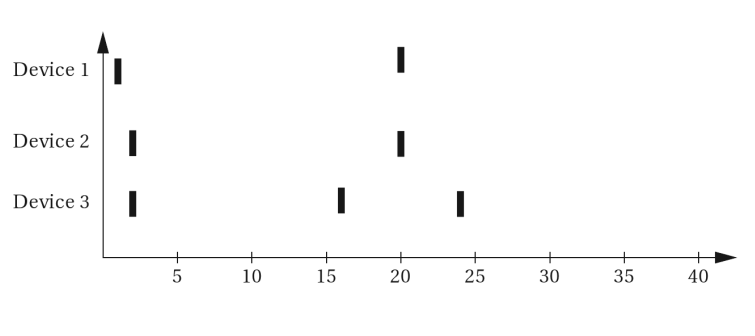
\includegraphics[width=\textwidth,keepaspectratio]{Q3-19}
		\caption{Device Interrupt Timing}
	\end{subfigure}
% Agents
\def\DA{Device 1}
\def\DB{Device 2}
\def\DC{Device 3}

	\begin{subfigure}[b]{\textwidth}
		\centering
% Diagram for Q3-19
\begin{tikzpicture}[every node/.style={font=\normalsize,minimum height=0.25cm,minimum width=0.5cm},]
	
	% Matrix
	\node [matrix, very thin,column sep=1.3cm,row sep=0.005cm] (matrix) at (0,0) {
	  & \node(0,0) (\DA) {}; & & \node(0,0) (\DB) {}; &  & \node(0,0) (\DC) {}; & \\
	  \node(0,0) (tt left) {}; & & & & & & \node(0,0) (tt right) {};\\
	  \node(0,0) (t0 left) {}; & & & & & & \node(0,0) (t0 right) {};\\
	  & \node(0,0) (\DA 1) {}; & & \node(0,0) (\DB 1) {}; & & \node(0,0) (\DC 1) {}; &\\
	  & \node(0,0) (\DA 2) {}; & & \node(0,0) (\DB 2) {}; & & \node(0,0) (\DC 2) {}; &\\
	  & \node(0,0) (\DA 3) {}; & & \node(0,0) (\DB 3) {}; & & \node(0,0) (\DC 3) {}; & \\
	  & \node(0,0) (\DA 4) {}; & & \node(0,0) (\DB 4) {}; & & \node(0,0) (\DC 4) {}; & \\
	  \node(0,0) (t1 left) {}; & & & & & & \node(0,0) (t1 right) {};\\
	  & \node(0,0) (\DA 6) {}; & & \node(0,0) (\DB 6) {}; & & \node(0,0) (\DC 6) {}; & \\
	  & \node(0,0) (\DA 7) {}; & & \node(0,0) (\DB 7) {}; & & \node(0,0) (\DC 7) {}; & \\
	  & \node(0,0) (\DA 8) {}; & & \node(0,0) (\DB 8) {}; & & \node(0,0) (\DC 8) {}; & \\
	  & \node(0,0) (\DA 9) {}; & & \node(0,0) (\DB 9) {}; & & \node(0,0) (\DC 9) {}; & \\ 
	  \node(0,0) (t2 left) {}; & & & & & & \node(0,0) (t2 right) {};\\
	  & \node(0,0) (\DA 11) {}; & & \node(0,0) (\DB 11) {}; & & \node(0,0) (\DC 11) {}; & \\
	  & \node(0,0) (\DA 12) {}; & & \node(0,0) (\DB 12) {}; & & \node(0,0) (\DC 12) {}; & \\
	  & \node(0,0) (\DA 13) {}; & & \node(0,0) (\DB 13) {}; & & \node(0,0) (\DC 13) {}; & \\
	  & \node(0,0) (\DA 14) {}; & & \node(0,0) (\DB 14) {}; & & \node(0,0) (\DC 14) {}; & \\  
	  \node(0,0) (t3 left) {}; & & & & & & \node(0,0) (t3 right) {};\\
	  & \node(0,0) (\DA 16) {}; & & \node(0,0) (\DB 16) {}; & & \node(0,0) (\DC 16) {}; & \\
	  & \node(0,0) (\DA 17) {}; & & \node(0,0) (\DB 17) {}; & & \node(0,0) (\DC 17) {}; & \\
	  & \node(0,0) (\DA 18) {}; & & \node(0,0) (\DB 18) {}; & & \node(0,0) (\DC 18) {}; & \\
	  & \node(0,0) (\DA 19) {}; & & \node(0,0) (\DB 19) {}; & & \node(0,0) (\DC 19) {}; & \\  
	  \node(0,0) (t4 left) {}; &\node(0,0) (\DA 20) {};  & & & & \node(0,0) (\DC 20) {}; & \node(0,0) (t4 right) {};\\
	  & \node(0,0) (\DA 21) {}; & & \node(0,0) (\DB 21) {}; & & \node(0,0) (\DC 21) {}; & \\
	  & \node(0,0) (\DA 22) {}; & & \node(0,0) (\DB 22) {}; & & \node(0,0) (\DC 22) {}; & \\
	  & \node(0,0) (\DA 23) {}; & & \node(0,0) (\DB 23) {}; & & \node(0,0) (\DC 23) {}; & \\
	  & \node(0,0) (\DA 24) {}; & & \node(0,0) (\DB 24) {}; & & \node(0,0) (\DC 24) {}; & \\  
	  \node(0,0) (t5 left) {}; & & & & & & \node(0,0) (t5 right) {};\\
	  & \node(0,0) (\DA 26) {}; & & \node(0,0) (\DB 26) {}; & & \node(0,0) (\DC 26) {}; & \\
	  & \node(0,0) (\DA 27) {}; & & \node(0,0) (\DB 27) {}; & & \node(0,0) (\DC 27) {}; & \\
	  & \node(0,0) (\DA 28) {}; & & \node(0,0) (\DB 28) {}; & & \node(0,0) (\DC 28) {}; & \\
	  & \node(0,0) (\DA 29) {}; & & \node(0,0) (\DB 29) {}; & & \node(0,0) (\DC 29) {}; & \\  
	  \node(0,0) (t6 left) {}; & & & & & & \node(0,0) (t6 right) {};\\
	  & \node(0,0) (\DA 31) {}; & & \node(0,0) (\DB 31) {}; & & \node(0,0) (\DC 31) {}; & \\
	  & \node(0,0) (\DA 32) {}; & & \node(0,0) (\DB 32) {}; & & \node(0,0) (\DC 32) {}; & \\
	  & \node(0,0) (\DA 33) {}; & & \node(0,0) (\DB 33) {}; & & \node(0,0) (\DC 33) {}; & \\
	  & \node(0,0) (\DA 34) {}; & & \node(0,0) (\DB 34) {}; & & \node(0,0) (\DC 34) {}; & \\  
	  \node(0,0) (t7 left) {}; & & & & & & \node(0,0) (t7 right) {};\\
	  & \node(0,0) (\DA 36) {}; & & \node(0,0) (\DB 36) {}; & & \node(0,0) (\DC 36) {}; & \\
	  & \node(0,0) (\DA 37) {}; & & \node(0,0) (\DB 37) {}; & & \node(0,0) (\DC 37) {}; & \\
	  & \node(0,0) (\DA 38) {}; & & \node(0,0) (\DB 38) {}; & & \node(0,0) (\DC 38) {}; & \\
	  & \node(0,0) (\DA 39) {}; & & \node(0,0) (\DB 39) {}; & & \node(0,0) (\DC 39) {}; & \\  
	  \node(0,0) (t8 left) {}; & & & & & & \node(0,0) (t8 right) {};\\
	  & \node(0,0) (\DA 41) {}; & & \node(0,0) (\DB 41) {}; & & \node(0,0) (\DC 41) {}; & \\
	  };

	% Agents labels
	\fill 
	(\DA) node[draw,fill=gray] {\DA}
	(\DB) node[draw,fill=gray] {\DB}
	(\DC) node[draw,fill=gray] {\DC};
	
	% Horizontal time lines
	\draw [dotted] 
	  (t0 left) -- (t0 right) node[right] {$0$}
	  (t1 left) -- (t1 right) node[right] {$5$}
	  (t2 left) -- (t2 right) node[right] {$10$}
	  (t3 left) -- (t3 right) node[right] {$15$}
	  (t4 left) -- (t4 right) node[right] {$20$}
	  (t5 left) -- (t5 right) node[right] {$25$}
	  (t6 left) -- (t6 right) node[right] {$30$}
	  (t7 left) -- (t7 right) node[right] {$35$}
	  (t8 left) -- (t8 right) node[right] {$40$};
	
	% Vertical lifelines
	\draw [dashed] 
	  (\DA.south) -- (\DA 41)
	  (\DB.south) -- (\DB 41)
	  (\DC.south) -- (\DC 41);
	
	% Blocks (Handler Execution)
	\filldraw[fill=blue!20]
	  (\DA 1.north west) rectangle (\DA 6.north east)
	  (\DB 6.north west) rectangle (\DB 11.north east)
	  (\DC 11.north west) rectangle (\DC 16.north east)
	  (\DC 16.north west) rectangle (\DC 20.mid east)
	  (\DA 20.mid west) rectangle (\DA 26.north east)
	  (\DB 26.north west) rectangle (\DB 31.north east)
	  (\DC 31.north west) rectangle (\DC 32.north east)
	  (\DC 32.north west) rectangle (\DC 37.north east);
	
	% Horizontal flows (Monetary interactions)
	\draw [-latex] (\DA 6.north east) -- (\DB 6.north west);
	\draw [-latex] (\DB 11.north east) -- (\DC 11.north west);
	\draw [-latex] (\DC 20.mid west) -- (\DA 20.mid east);
	\draw [-latex] (\DA 26.north east) -- (\DB 26.north west);
	\draw [-latex] (\DB 31.north east) -- (\DC 31.north west);
	
	\end{tikzpicture}
\caption{Sequence Diagram for Interrupt Handlers}
\end{subfigure}
\end{figure}


% -----------------------------------------------%
%  \begin{figure}[htbp]
%   \centering
%   \includegraphics[width=4.0in,keepaspectratio]{E-Field}
%   \caption{\small{ The E-Field pattern produced by the initial code. }}
%   \label{fig:E-Field}
%   \end{figure}
%  \begin{figure}[htbp]
%   \centering
%   \includegraphics[width=4.0in,keepaspectratio]{Power}
%   \caption{\small{ The normalized power pattern of the system.  }}
%   \label{fig:Power}
%   \end{figure}

\label{end}\end{document}


